\documentclass{article}

\usepackage{tikz}

\pagenumbering{gobble}

\begin{document}

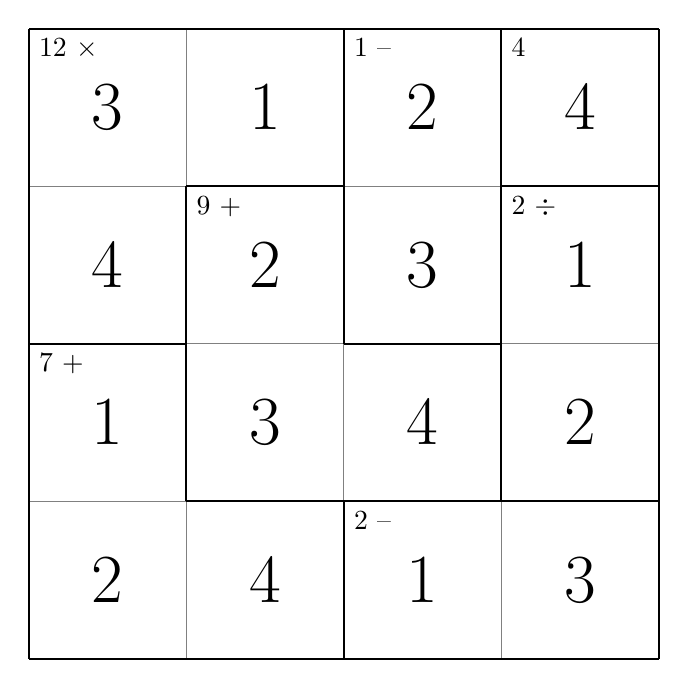
\begin{tikzpicture}
	
	% The Grid
	\draw[step=2cm,gray,very thin] (0,0) grid (8,8);

	% id: 1
	\draw[thick] (0, 8) -- (0, 6);
	\draw[thick] (2, 8) -- (0, 8) node[anchor=north west] {12 $\times$};
	\draw[thick] (2, 6) -- (4, 6);
	\draw[thick] (4, 6) -- (4, 8);
	\draw[thick] (4, 8) -- (2, 8);
	\draw[thick] (0, 6) -- (0, 4);
	\draw[thick] (0, 4) -- (2, 4);
	\draw[thick] (2, 4) -- (2, 6);

	% id: 2
	\draw[thick] (4, 8) -- (4, 6);
	\draw[thick] (6, 6) -- (6, 8);
	\draw[thick] (6, 8) -- (4, 8) node[anchor=north west] {1 --};
	\draw[thick] (4, 6) -- (4, 4);
	\draw[thick] (4, 4) -- (6, 4);
	\draw[thick] (6, 4) -- (6, 6);

	% id: 3
	\draw[thick] (6, 8) -- (6, 6);
	\draw[thick] (6, 6) -- (8, 6);
	\draw[thick] (8, 6) -- (8, 8);
	\draw[thick] (8, 8) -- (6, 8) node[anchor=north west] {4  };

	% id: 4
	\draw[thick] (2, 6) -- (2, 4);
	\draw[thick] (4, 4) -- (4, 6);
	\draw[thick] (4, 6) -- (2, 6) node[anchor=north west] {9 +};
	\draw[thick] (2, 4) -- (2, 2);
	\draw[thick] (2, 2) -- (4, 2);
	\draw[thick] (4, 2) -- (6, 2);
	\draw[thick] (6, 2) -- (6, 4);
	\draw[thick] (6, 4) -- (4, 4);

	% id: 5
	\draw[thick] (6, 6) -- (6, 4);
	\draw[thick] (8, 4) -- (8, 6);
	\draw[thick] (8, 6) -- (6, 6) node[anchor=north west] {2 $\div$};
	\draw[thick] (6, 4) -- (6, 2);
	\draw[thick] (6, 2) -- (8, 2);
	\draw[thick] (8, 2) -- (8, 4);

	% id: 6
	\draw[thick] (0, 4) -- (0, 2);
	\draw[thick] (2, 2) -- (2, 4);
	\draw[thick] (2, 4) -- (0, 4) node[anchor=north west] {7 +};
	\draw[thick] (0, 2) -- (0, 0);
	\draw[thick] (0, 0) -- (2, 0);
	\draw[thick] (2, 0) -- (4, 0);
	\draw[thick] (4, 0) -- (4, 2);
	\draw[thick] (4, 2) -- (2, 2);

	% id: 7
	\draw[thick] (4, 2) -- (4, 0);
	\draw[thick] (4, 0) -- (6, 0);
	\draw[thick] (6, 2) -- (4, 2) node[anchor=north west] {2 --};
	\draw[thick] (6, 0) -- (8, 0);
	\draw[thick] (8, 0) -- (8, 2);
	\draw[thick] (8, 2) -- (6, 2);

	% Solution
	\draw (1,7) node[anchor=center] {\Huge 3};
	\draw (3,7) node[anchor=center] {\Huge 1};
	\draw (5,7) node[anchor=center] {\Huge 2};
	\draw (7,7) node[anchor=center] {\Huge 4};
	\draw (1,5) node[anchor=center] {\Huge 4};
	\draw (3,5) node[anchor=center] {\Huge 2};
	\draw (5,5) node[anchor=center] {\Huge 3};
	\draw (7,5) node[anchor=center] {\Huge 1};
	\draw (1,3) node[anchor=center] {\Huge 1};
	\draw (3,3) node[anchor=center] {\Huge 3};
	\draw (5,3) node[anchor=center] {\Huge 4};
	\draw (7,3) node[anchor=center] {\Huge 2};
	\draw (1,1) node[anchor=center] {\Huge 2};
	\draw (3,1) node[anchor=center] {\Huge 4};
	\draw (5,1) node[anchor=center] {\Huge 1};
	\draw (7,1) node[anchor=center] {\Huge 3};

\end{tikzpicture}

\end{document}

